\documentclass[a4paper,12pt,titlepage]{article}					% unlike report, article doesn't have \chapter

\usepackage[T1]{fontenc}									% exit font codec
\usepackage[utf8]{inputenc}								% applemac for accent characters on Mac, utf8 or others available
\usepackage[english]{babel}								% typographical elements for the chosen language
\usepackage{amsmath,amsfonts,amssymb,amsthm,dsfont}		% mathematical symbols and characters
\usepackage{graphicx}									% insert figures
\usepackage{indentfirst}									% indent first line of a section
\usepackage{microtype}									% improve lines filling
\usepackage{hyperref} 									% clickable elements
\hypersetup{colorlinks=true,linkcolor=blue,linktocpage}			% options for clickable index
\usepackage{lipsum}										% fake text generator
\usepackage{mathtools}									% useful for \vdotswithin command
\usepackage{fancyhdr}									% header/footer
\usepackage{comment}									% comment block
\usepackage{textcomp}									% \textsuperscript{TM} or \texttrademark and \textregistered\textcopyright or \sffamily\textregistered\textcopyright
\usepackage[scale=0.77]{geometry}							% scale factor for the entire document
\usepackage{fancyvrb}									% Verbatim block (different from verbatim) works with tabs
\fvset{tabsize=4,fontsize=\small}							% option for fancyvrb
\usepackage{upquote}									% fix quotes with verbatim/Verbatim
%\usepackage{fvextra}
\usepackage{subfig}										% for the subfloat environment
\usepackage{caption}									% required by subfig package


\pagestyle{fancy}										% document oneside
\lhead{\nouppercase\leftmark}
\rhead{\nouppercase\rightmark}
\cfoot{\thepage}

\title{$Simple_{X}^{n}$ module\\\begin{small}IN480 course~\cite{Paoluzzi:coursewebpage}\end{small}}
\author{Fabio Fatelli \and Emanuele Loprevite}

% ------- BEGIN DOCUMENT -------
\begin{document}

\maketitle

\tableofcontents
\thispagestyle{plain}

\clearpage

% ------- INTRODUCTION -------
\section{Introduction}
The $Simple^n_X$ library, named \textbf{simplexn} within the Python version of the LARCC framework, provides combinatorial algorithms for some basic functions of geometric modelling with simplicial complexes. In particular, provides the efficient creation of simplicial complexes generated by simplicial complexes of lower dimension, the production of simplicial grids of any dimension, and the extraction of facets (i.e. of $(d-1)$-faces) of complexes of $d$-simplices.~\cite{Paoluzzi:simplexn}

\subsection{Requirements}
There is no need to install extra packages to run the Julia code, it is sufficient loading the built-in package \emph{Combinatorics.jl} (i.e. \texttt{using Combinatorics}); however, in order to be able to make the graphs it is necessary to install the package \emph{Plots.jl}~\cite{Julia:plots} (i.e. \texttt{Pkg.add(\textquotedbl Plots\textquotedbl)}) with the preferred backend (for example \texttt{Pkg.add(\textquotedbl GR\textquotedbl)}) and load them (i.e. \texttt{using Plots} and \texttt{gr()}).

Four processors were used (\texttt{addprocs(4)} at startup) for all the tests, five REPL included; for the tests environment it is necessary to load \texttt{using Base.Test}.

To execute the speedup code it is required the following:
\begin{Verbatim}
using Plots
Plots.scalefontsizes(0.7)
gr() # loading backend

VOID = [Int64[]],[[0]] # the empty simplicial model
nt, N = 7, 5

# Compute the execution mean time
function timing(f::Function,x,n::Int64)
	t = Array{Float64}(n)
	f(x...)
	for k in 1:n
		t[k] = @elapsed f(x...)
	end
	return mean(t)
end

# Create the plots
function plotting(name::String,timeS::Array{Float64,1},timeP::Array{Float64,1})
	l = max(length(timeS),length(timeP))+1
	s, p, xlb, ylb, DPI = "Serial", "Parallel", "Input", "Time (seconds)", 150
	p1 = plot(timeS,label=s,title=name)
	p2 = plot(timeP,label=p)
	p3 = plot([timeS,timeP],label=[s,p])
	plot(p1,p2,p3,xlims=(1,l),xlabel=xlb,ylabel=ylb,dpi=1.5*DPI,legend=:topleft)
end
\end{Verbatim}

\subsection{API}
In Python the dependencies were the following (see figure~\ref{fig:dependenciesGraph}):

\begin{figure}[h]
\centering
\subfloat[][\emph{larExtrude1, larSimplexGrid1, and larSimplexFacets}]
	{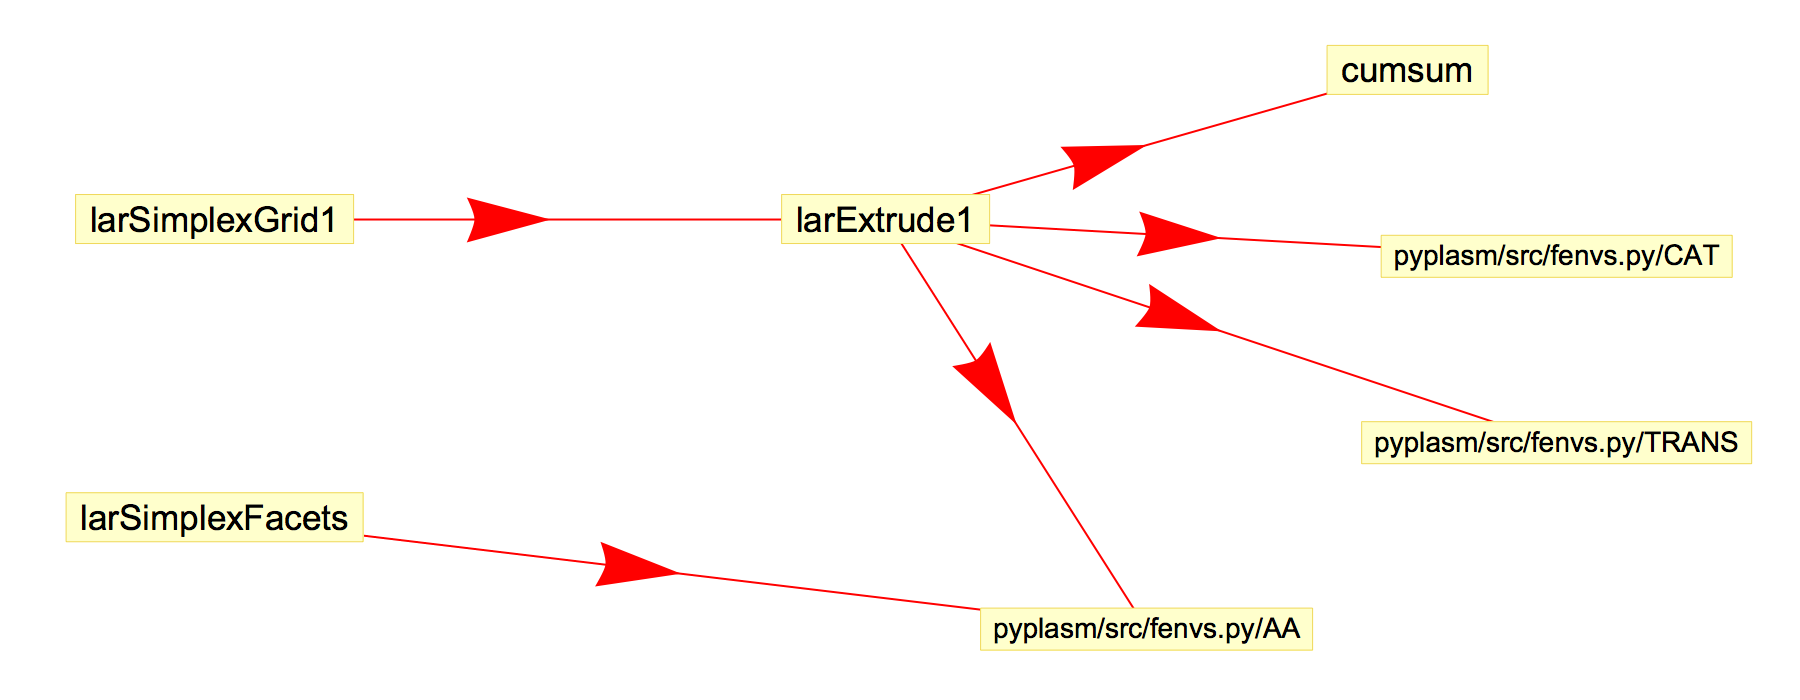
\includegraphics[scale=0.245]{figures/Graph1}} \quad
\subfloat[][\emph{quads2tria}]
	{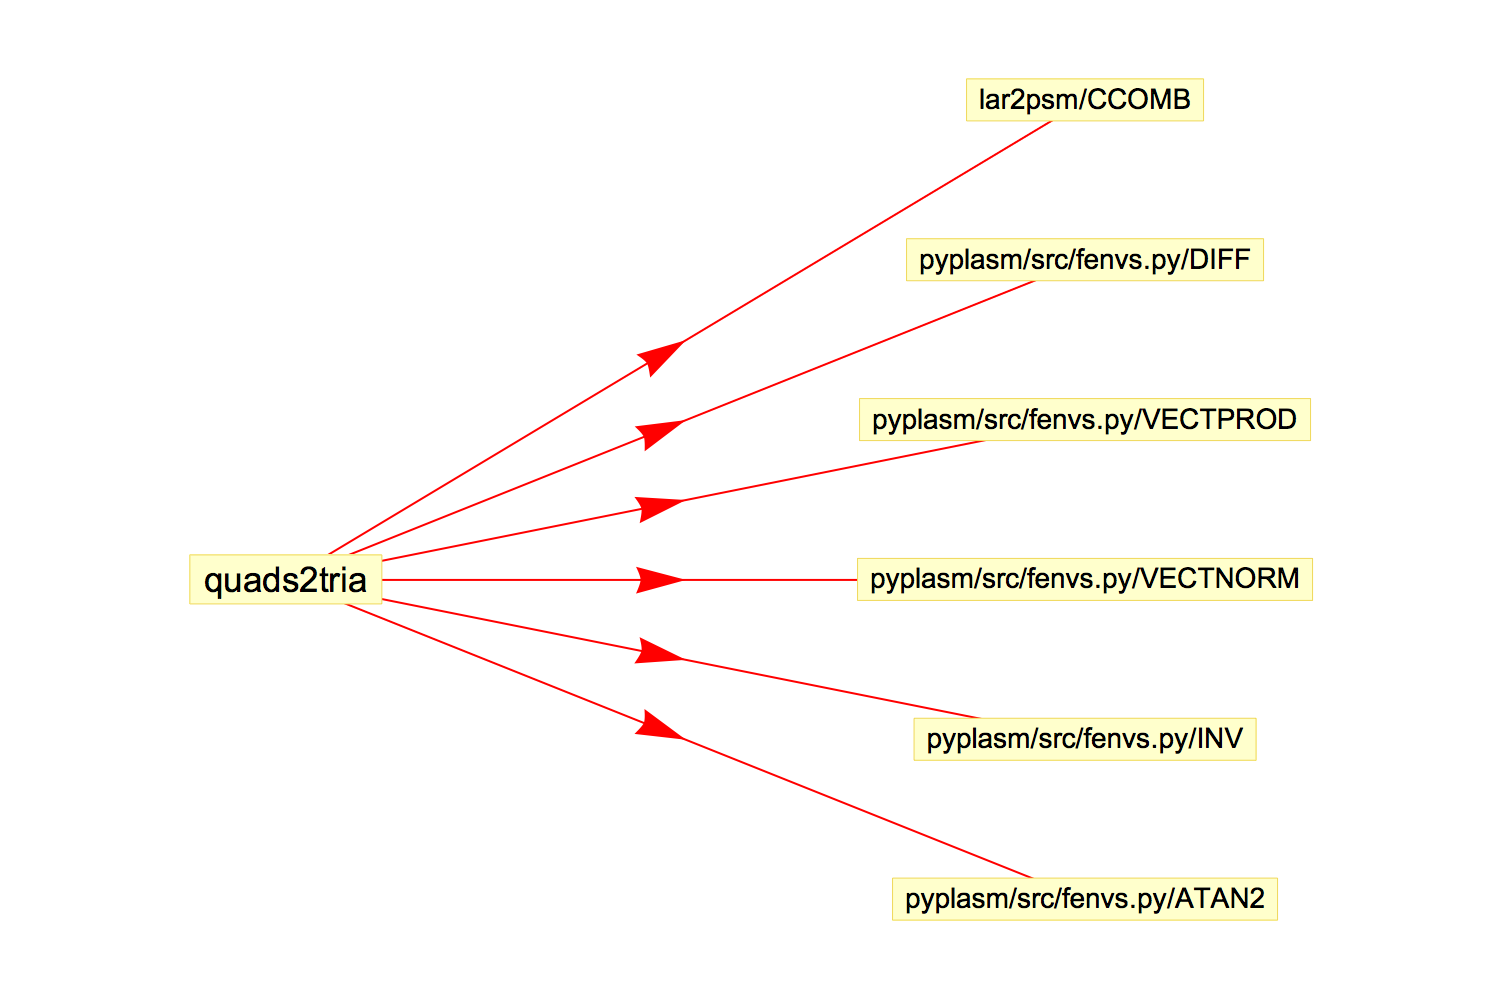
\includegraphics[scale=0.245]{figures/Graph2}}
\caption{Dependencies graph}
\label{fig:dependenciesGraph}
\end{figure}

In the Julia translation all the dependencies have been removed, so now there is only \texttt{larSimplexGrid1} calling \texttt{larExtrude1}; moreover, \texttt{larSimplexFacets} uses the function \texttt{combinations} which is in the built-in package \emph{Combinatorics.jl} .\\

The Julia API describes the serial functions but it is the same for the parallel ones, the only difference is the names beginning with a \texttt{p}.\\

\texttt{larExtrude1\{T<:Real\}(model::Tuple\{Array\{Array\{T,1\},1\},Array\{Array\{Int64,1\},1\}\},\\pattern::Array\{Int64,1\})}
\\
\emph{Description}: this function generates the output model vertices in a multiple extrusion of a LAR model.
\\
\emph{Input}: \texttt{model} contains a pair (V, FV), where V is the array of input vertices, and FV is the array of $d$-cells (given as arrays of vertex indices) providing the input representation of a LAR cellular complex.
\texttt{pattern} is an array of integers, whose absolute values provide the sizes of the ordered set of 1D (in local coords) subintervals specified by the pattern itself.
\\
\emph{Output}: it is a model representing the extrusion of the input \texttt{model}.
\\

\texttt{larSimplexGrid1(shape::Array\{Int64,1\})}
\\
\emph{Description}: this function generates the simplicial grids of any dimension and shape.
\\
\emph{Input}: \texttt{shape} is an array of integers used to specify the shape of the created array.
\\
\emph{Output}: it is a model that contains a pair (V, FV), where V is the array of input vertices, and FV is the array of $d$-cells (given as arrays of vertex indices) providing the input representation of a LAR cellular complex.
\\

\texttt{larSimplexFacets(simplices::Array\{Array\{Int64,1\},1\})}
\\
\emph{Description}: this function provides the extraction of non-oriented $(d-1)$-facets of $d$-dimensional simplices.
\\
\emph{Input}: \texttt{simplices} is the array of $d$-cells (given as arrays of vertex indices) providing the input representation of a LAR cellular complex.
\\
\emph{Output}: it is an array of $d$-cells of integers, i.e. the input LAR representation of the topology of a cellular complex.
\\

\texttt{quads2tria\{T<:Real\}(model::Tuple\{Array\{Array\{T,1\},1\},Array\{Array\{Int64,1\},1\}\})}
\\
\emph{Description}: this function gives the conversion of a LAR boundary representation (B-Rep), i.e. a LAR model \textbf{\textsc{V, FV}} made of 2D faces, usually quads but also general polygons, into a LAR model \textbf{\textsc{verts, triangles}} made by triangles.
\\
\emph{Input}: \texttt{model} contains a pair (V, FV), where V is the array of input vertices, and FV is the array of $d$-cells (given as arrays of vertex indices) providing the input representation of a LAR cellular complex.
\\
\emph{Output}: it is a model that contains a pair (V, triangles) representing the triangulation of the input \texttt{model}.


% ------- IMPLEMENTATION -------
\section{Implementation}
All the code in this section works with a simple copy and paste in Julia REPL; however, if a code block starts in a page and ends at the following one, it is required to pay attention at the numbers and headers of the pages.

Moreover, there are some comments, which could be useful, left on purpose in the code.

\subsection{larExtrude1}
This function generates the output model vertices in a multiple extrusion of a LAR model.

\subsubsection{Python code}
\begin{verbatim}
def larExtrude1(model,pattern):
    V, FV = model
    d, m = len(FV[0]), len(pattern)
    coords = list(cumsum([0]+(AA(ABS)(pattern))))
    offset, outcells, rangelimit = len(V), [], d*m
    for cell in FV:
        tube = [v + k*offset for k in range(m+1) for v in cell]
        cellTube = [tube[k:k+d+1] for k in range(rangelimit)]
        outcells += [reshape(cellTube, newshape=(m,d,d+1)).tolist()]
        
    outcells = AA(CAT)(TRANS(outcells))
    cellGroups = [group for k,group in enumerate(outcells) if pattern[k]>0]
    outVertices = [v+[z] for z in coords for v in V]
    outModel = outVertices, CAT(cellGroups)
    return outModel
\end{verbatim}

\subsubsection{Julia code - serial}
During the translation a part of the code is changed to use a matrix for \texttt{outcells} instead of a list of lists of lists.

\begin{Verbatim}
# Generation of the output model vertices in a multiple extrusion of a LAR model
function larExtrude1{T<:Real}(model::Tuple{Array{Array{T,1},1},Array{
  Array{Int64,1},1}},pattern::Array{Int64,1})
	V, FV = model
	d, m = length(FV[1]), length(pattern)
	coords = cumsum(append!([0],abs.(pattern))) # built-in function cumsum
	offset, outcells, rangelimit = length(V), Array{Int64}(m,0), d*m
	for cell in FV
		tube = [v+k*offset for k in 0:m for v in cell]
		celltube = Int64[]
		for k in 1:rangelimit
			append!(celltube,tube[k:k+d])
		end
		outcells = hcat(outcells,reshape(celltube,d*(d+1),m)')
	end
	cellGroups = Int64[]
	for k in 1:m
		if pattern[k]>0
			cellGroups = vcat(cellGroups,outcells[k,:])
		end
	end
	outVertices = [vcat(v,z) for z in coords for v in V]
	outCellGroups = Array{Int64,1}[]
	for k in 1:d+1:length(cellGroups)
		append!(outCellGroups,[cellGroups[k:k+d]])
	end
	return outVertices, outCellGroups
end
\end{Verbatim}

\subsubsection{Parallel optimization}
Every single \texttt{for} loop has been parallelized with the \texttt{@parallel} macro, using also \texttt{@sync} where needed.

\texttt{outVertices} is computed as soon as possible with the help of the macro \texttt{@spawn} because it is independent from the rest of the code.
The \texttt{outcells} array is changed into a \texttt{SharedArray} to be available on all the processors, and the dimension is established a priori to preserve the correct order of the computation and avoid the possible random order due to the \texttt{hcat} in the \texttt{@parallel for}; same as for \texttt{cellGroups}, and in this case a SharedArray \texttt{p} has been used to remove the \texttt{if} inside the loop which would have invalidated the parallelization.


\subsubsection{Julia code - parallel}
\begin{Verbatim}
# Generation of the output model vertices in a multiple extrusion of a LAR model
@everywhere function plarExtrude1{T<:Real}(model::Tuple{Array{Array{T,1},1},Array{
  Array{Int64,1},1}}, pattern::Array{Int64,1})
	V, FV = model
	d, m = length(FV[1]), length(pattern)
	dd1 = d*(d+1)
	coords = cumsum(append!([0],abs.(pattern))) # built-in function cumsum
	outVertices = @spawn [vcat(v,z) for z in coords for v in V]
	offset,outcells,rangelimit=length(V),SharedArray{Int64}(m,dd1*length(FV)),d*m
	@sync @parallel for j in 1:length(FV)
		tube = [v+k*offset for k in 0:m for v in FV[j]]
		celltube = Int64[]
		celltube = @sync @parallel (append!) for k in 1:rangelimit
			tube[k:k+d]
		end
		outcells[:,(j-1)*dd1+1:(j-1)*dd1+dd1] = reshape(celltube,dd1,m)'
	end
	p = convert(SharedArray,find(x->x>0,pattern))
	cellGroups = SharedArray{Int64}(length(p),size(outcells)[2])
	@sync @parallel for k in 1:length(p)
		cellGroups[k,:] = outcells[p[k],:]
	end
	cellGroupsL = vec(cellGroups')
	outCellGroups = Array{Int64,1}[]
	outCellGroups = @parallel (append!) for k in 1:d+1:length(cellGroupsL)
			[cellGroupsL[k:k+d]]
		end
	return fetch(outVertices), outCellGroups
end
\end{Verbatim}

\subsubsection{Unit tests code}
\emph{- Serial Tests -}

\begin{Verbatim}
@testset "larExtrude1" begin
	VOID = [Int64[]],[[0]] # the empty simplicial model
	pattern1 = [1,-1]
	model1 = larExtrude1(VOID,pattern1) # 1D
	@test typeof(model1) == Tuple{Array{Array{Int64,1},1},Array{Array{Int64,1},1}}
	@test length(model1[1]) == length(pattern1)+1 # num of vertices, no rep
	@test length(model1[2]) == length(filter(x->x>0,pattern1)) #num of 1D-simplices
	
	pattern2 = [1,1,1,-1]
	model2 = larExtrude1(VOID,pattern2) # 1D
	@test typeof(model2) == Tuple{Array{Array{Int64,1},1},Array{Array{Int64,1},1}}
	@test length(model2[1]) == length(pattern2)+1 # num of vertices, no rep
	@test length(model2[2]) == length(filter(x->x>0,pattern2)) #num of 1D-simplices
	
	pattern3 = [1,1,1,1,1,-1]
	model3 = larExtrude1(VOID,pattern3) # 1D
	@test typeof(model3) == Tuple{Array{Array{Int64,1},1},Array{Array{Int64,1},1}}
	@test length(model3[1]) == length(pattern3)+1 # num of vertices, no rep
	@test length(model3[2]) == length(filter(x->x>0,pattern3)) #num of 1D-simplices
	
	model1 = larExtrude1(model1,pattern1) # 2D
	@test typeof(model1) == Tuple{Array{Array{Int64,1},1},Array{Array{Int64,1},1}}
	@test length(model1[1]) == (length(pattern1)+1)^2 # num of vertices, no rep
	@test length(model1[2]) == 2*length(filter(x->x>0,pattern1))^2 #num of 2D-simplices
	
	model2 = larExtrude1(model2,pattern2) # 2D
	@test typeof(model2) == Tuple{Array{Array{Int64,1},1},Array{Array{Int64,1},1}}
	@test length(model2[1]) == (length(pattern2)+1)^2 # num of vertices, no rep
	@test length(model2[2]) == 2*length(filter(x->x>0,pattern2))^2 #num of 2D-simplices
	
	model3 = larExtrude1(model3,pattern3) # 2D
	@test typeof(model3) == Tuple{Array{Array{Int64,1},1},Array{Array{Int64,1},1}}
	@test length(model3[1]) == (length(pattern3)+1)^2 # num of vertices, no rep
	@test length(model3[2]) == 2*length(filter(x->x>0,pattern3))^2 #num of 2D-simplices
	
	model1 = larExtrude1(model1,pattern1) # 3D
	@test typeof(model1) == Tuple{Array{Array{Int64,1},1},Array{Array{Int64,1},1}}
	@test length(model1[1]) == (length(pattern1)+1)^3 # num of vertices, no rep
	@test length(model1[2]) == 6*length(filter(x->x>0,pattern1))^3 #num of 3D-simplices
	
	model2 = larExtrude1(model2,pattern2) # 3D
	@test typeof(model2) == Tuple{Array{Array{Int64,1},1},Array{Array{Int64,1},1}}
	@test length(model2[1]) == (length(pattern2)+1)^3 # num of vertices, no rep
	@test length(model2[2]) == 6*length(filter(x->x>0,pattern2))^3 #num of 3D-simplices
	
	model3 = larExtrude1(model3,pattern3) # 3D
	@test typeof(model3) == Tuple{Array{Array{Int64,1},1},Array{Array{Int64,1},1}}
	@test length(model3[1]) == (length(pattern3)+1)^3 # num of vertices, no rep
	@test length(model3[2]) == 6*length(filter(x->x>0,pattern3))^3 #num of 3D-simplices
	
	model = ([[0.0,0],[0,1]],[[1,0],[1,1]]) # 2D with float
	@test typeof(model[1]) == Array{Array{Float64,1},1}
	model = larExtrude1(model,pattern1)
	@test typeof(model) == Tuple{Array{Array{Float64,1},1},Array{Array{Int64,1},1}}
end
\end{Verbatim}

\emph{- Parallel Tests -}

\begin{Verbatim}
@testset "plarExtrude1" begin
	VOID = [Int64[]],[[0]] # the empty simplicial model
	pattern1 = [1,-1]
	model1 = plarExtrude1(VOID,pattern1) # 1D
	@test typeof(model1) == Tuple{Array{Array{Int64,1},1},Array{Array{Int64,1},1}}
	@test length(model1[1]) == length(pattern1)+1 # num of vertices, no rep
	@test length(model1[2]) == length(filter(x->x>0,pattern1)) #num of 1D-simplices
	
	pattern2 = [1,1,1,-1]
	model2 = plarExtrude1(VOID,pattern2) # 1D
	@test typeof(model2) == Tuple{Array{Array{Int64,1},1},Array{Array{Int64,1},1}}
	@test length(model2[1]) == length(pattern2)+1 # num of vertices, no rep
	@test length(model2[2]) == length(filter(x->x>0,pattern2)) #num of 1D-simplices
	
	pattern3 = [1,1,1,1,1,-1]
	model3 = plarExtrude1(VOID,pattern3) # 1D
	@test typeof(model3) == Tuple{Array{Array{Int64,1},1},Array{Array{Int64,1},1}}
	@test length(model3[1]) == length(pattern3)+1 # num of vertices, no rep
	@test length(model3[2]) == length(filter(x->x>0,pattern3)) #num of 1D-simplices
	
	model1 = plarExtrude1(model1,pattern1) # 2D
	@test typeof(model1) == Tuple{Array{Array{Int64,1},1},Array{Array{Int64,1},1}}
	@test length(model1[1]) == (length(pattern1)+1)^2 # num of vertices, no rep
	@test length(model1[2]) == 2*length(filter(x->x>0,pattern1))^2 #num of 2D-simplices
	
	model2 = plarExtrude1(model2,pattern2) # 2D
	@test typeof(model2) == Tuple{Array{Array{Int64,1},1},Array{Array{Int64,1},1}}
	@test length(model2[1]) == (length(pattern2)+1)^2 # num of vertices, no rep
	@test length(model2[2]) == 2*length(filter(x->x>0,pattern2))^2 #num of 2D-simplices
	
	model3 = plarExtrude1(model3,pattern3) # 2D
	@test typeof(model3) == Tuple{Array{Array{Int64,1},1},Array{Array{Int64,1},1}}
	@test length(model3[1]) == (length(pattern3)+1)^2 # num of vertices, no rep
	@test length(model3[2]) == 2*length(filter(x->x>0,pattern3))^2 #num of 2D-simplices
	
	model1 = plarExtrude1(model1,pattern1) # 3D
	@test typeof(model1) == Tuple{Array{Array{Int64,1},1},Array{Array{Int64,1},1}}
	@test length(model1[1]) == (length(pattern1)+1)^3 # num of vertices, no rep
	@test length(model1[2]) == 6*length(filter(x->x>0,pattern1))^3 #num of 3D-simplices
	
	model2 = plarExtrude1(model2,pattern2) # 3D
	@test typeof(model2) == Tuple{Array{Array{Int64,1},1},Array{Array{Int64,1},1}}
	@test length(model2[1]) == (length(pattern2)+1)^3 # num of vertices, no rep
	@test length(model2[2]) == 6*length(filter(x->x>0,pattern2))^3 #num of 3D-simplices
	
	model3 = plarExtrude1(model3,pattern3) # 3D
	@test typeof(model3) == Tuple{Array{Array{Int64,1},1},Array{Array{Int64,1},1}}
	@test length(model3[1]) == (length(pattern3)+1)^3 # num of vertices, no rep
	@test length(model3[2]) == 6*length(filter(x->x>0,pattern3))^3 #num of 3D-simplices
	
	model = ([[0.0,0],[0,1]],[[1,0],[1,1]]) # 2D with float
	@test typeof(model[1]) == Array{Array{Float64,1},1}
	model = plarExtrude1(model,pattern1)
	@test typeof(model) == Tuple{Array{Array{Float64,1},1},Array{Array{Int64,1},1}}
end
\end{Verbatim}

\subsubsection{Speedup script code}
\begin{Verbatim}
timeSer = [timing(larExtrude1,[VOID,repmat([1,2,3,4],k^4)],nt) for k in 1:2*N]
timePar = [timing(plarExtrude1,[VOID,repmat([1,2,3,4],k^4)],nt) for k in 1:2*N]
plotting("larExtrude1",timeSer,timePar)
\end{Verbatim}

See figure~\ref{fig:larExtrude1}.

\begin{figure}[h]
\centering
\subfloat[][\emph{Serial}]
	{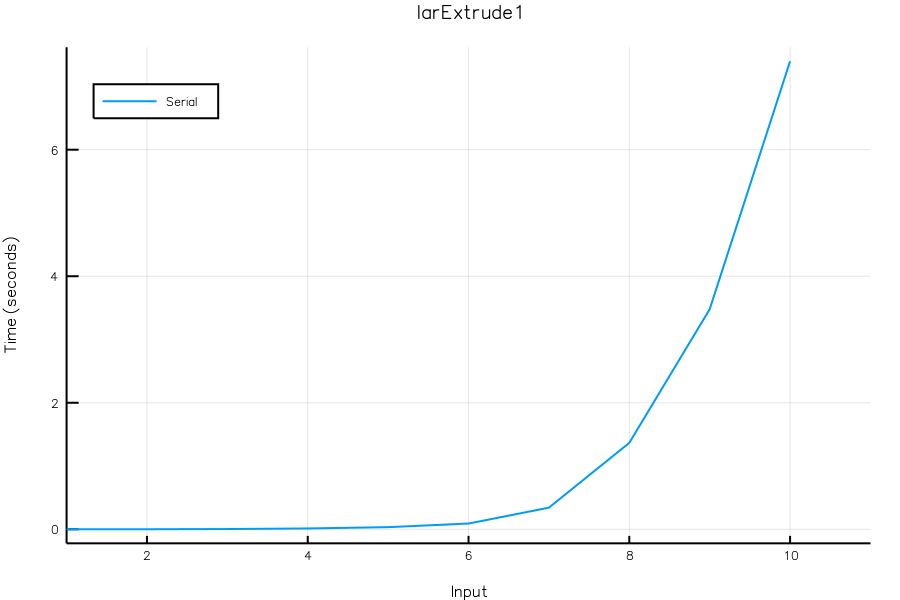
\includegraphics[scale=0.245]{figures/larExtrude1serial}} \quad
\subfloat[][\emph{Parallel}]
	{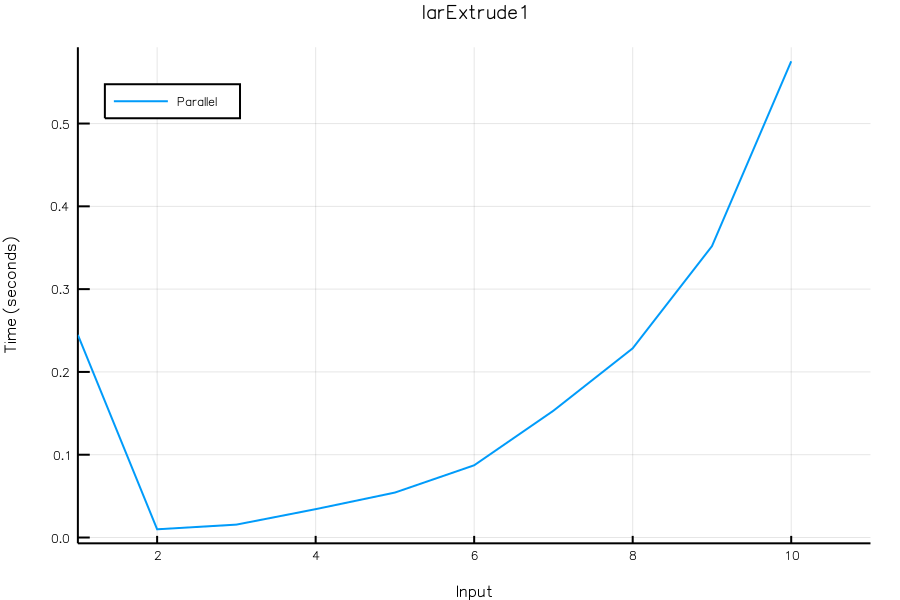
\includegraphics[scale=0.245]{figures/larExtrude1parallel}} \\
\subfloat[][\emph{Both}]
	{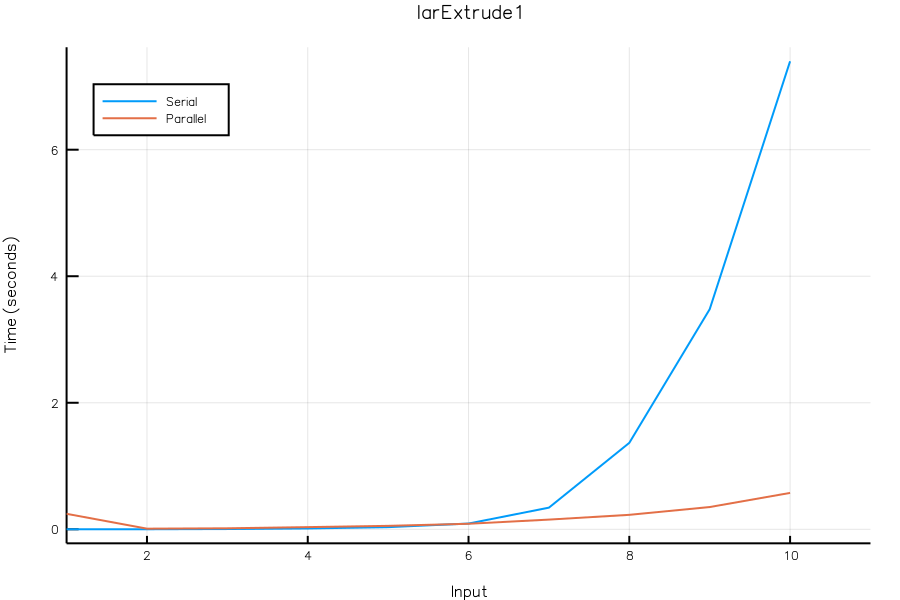
\includegraphics[scale=0.245]{figures/larExtrude1both}}
\caption{larExtrude1}
\label{fig:larExtrude1}
\end{figure}

\subsection{larSimplexGrid1}
This function generates the simplicial grids of any dimension and shape.

\subsubsection{Python code}
\begin{verbatim}
def larSimplexGrid1(shape):
    model = VOID
    for item in shape:
        model = larExtrude1(model,item*[1])
    return model
\end{verbatim}

\subsubsection{Julia code - serial}
\begin{Verbatim}
# Generation of simplicial grids of any dimension and shape
function larSimplexGrid1(shape::Array{Int64,1})
	model = [Int64[]],[[0]] # the empty simplicial model
	for item in shape
		model = larExtrude1(model,repmat([1],item))
	end
	return model
end
\end{Verbatim}

\subsubsection{Parallel optimization}
It is not possible to parallelize this function because every iteration of the loop requires the \texttt{model} that is computed in the previous one.
The only difference here is the addition of \texttt{@everywhere}.

\subsubsection{Julia code - parallel}
\begin{Verbatim}
# Generation of simplicial grids of any dimension and shape
@everywhere function plarSimplexGrid1(shape::Array{Int64,1})
	model = [Int64[]],[[0]] # the empty simplicial model
	for item in shape # no parallel
		model = plarExtrude1(model,repmat([1],item))
	end
	return model
end
\end{Verbatim}

\subsubsection{Unit tests code}
\emph{- Serial Tests -}

\begin{Verbatim}
@testset "larSimplexGrid1" begin
	shape = [3] # 1D
	model1 = larSimplexGrid1(shape)
	@test typeof(model1) == Tuple{Array{Array{Int64,1},1},Array{Array{Int64,1},1}}
	@test length(model1[1]) == shape[1]+1 # num of vertices, no rep
	@test length(model1[2]) == shape[1] # num of 1D-simplices
	
	shape = [3,5] # 2D
	model2 = larSimplexGrid1(shape)
	@test typeof(model2) == Tuple{Array{Array{Int64,1},1},Array{Array{Int64,1},1}}
	# (shape[1]+1)*(shape[2]+1)
	@test length(model2[1]) == prod(shape)+sum(shape)+1 # num of vertices, no rep
	@test length(model2[2]) == 2*prod(shape) # num of 2D-simplices
	
	shape = [3,5,7] # 3D
	model3 = larSimplexGrid1(shape)
	@test typeof(model3) == Tuple{Array{Array{Int64,1},1},Array{Array{Int64,1},1}}
	# (shape[1]+1)*(shape[2]+1)*(shape[3]+1); num of vertices, no rep
	@test length(model3[1]) == prod(shape)+sum(prod.(collect(combinations(shape,2))))
	  +sum(shape)+1
	@test length(model3[2]) == 6*prod(shape) # num of 3D-simplices
end
\end{Verbatim}

\emph{- Parallel Tests -}

\begin{Verbatim}
@testset "plarSimplexGrid1" begin
	shape = [3] # 1D
	model1 = plarSimplexGrid1(shape)
	@test typeof(model1) == Tuple{Array{Array{Int64,1},1},Array{Array{Int64,1},1}}
	@test length(model1[1]) == shape[1]+1 # num of vertices, no rep
	@test length(model1[2]) == shape[1] # num of 1D-simplices
	
	shape = [3,5] # 2D
	model2 = plarSimplexGrid1(shape)
	@test typeof(model2) == Tuple{Array{Array{Int64,1},1},Array{Array{Int64,1},1}}
	# (shape[1]+1)*(shape[2]+1)
	@test length(model2[1]) == prod(shape)+sum(shape)+1 # num of vertices, no rep
	@test length(model2[2]) == 2*prod(shape) # num of 2D-simplices
	
	shape = [3,5,7] # 3D
	model3 = plarSimplexGrid1(shape)
	@test typeof(model3) == Tuple{Array{Array{Int64,1},1},Array{Array{Int64,1},1}}
	# (shape[1]+1)*(shape[2]+1)*(shape[3]+1); num of vertices, no rep
	@test length(model3[1]) == prod(shape)+sum(prod.(collect(combinations(shape,2))))
	  +sum(shape)+1
	@test length(model3[2]) == 6*prod(shape) # num of 3D-simplices
end
\end{Verbatim}

\subsubsection{Speedup script code}
The code of the two versions is identical so it does not make sense to check the speedup.


\subsection{larSimplexFacets}
This function provides the extraction of non-oriented $(d-1)$-facets of $d$-dimensional simplices.

\subsubsection{Python code}
\begin{verbatim}
def larSimplexFacets(simplices):
    out = []
    d = len(simplices[0])
    for simplex in simplices:
        out += AA(sorted)([simplex[0:k]+simplex[k+1:d] for k in range(d)])
    out = set(AA(tuple)(out))
    return  sorted(out)
\end{verbatim}

\subsubsection{Julia code - serial}
\begin{Verbatim}
# Extraction of non-oriented (d-1)-facets of d-dimensional simplices
using Combinatorics # for combinations() function

function larSimplexFacets(simplices::Array{Array{Int64,1},1})
	out = Array{Int64,1}[]
	d = length(simplices[1])
	for simplex in simplices
		append!(out,collect(combinations(simplex,d-1)))
	end
	return sort!(unique(out),lt=lexless)
end
\end{Verbatim}

\subsubsection{Parallel optimization}
Here, other than the usual addition of \texttt{@everywhere}, the \texttt{@parallel} was used to split the computation of the \texttt{for} among multiple processors.
The \texttt{return} automatically waits the end of the computation.

\subsubsection{Julia code - parallel}
\begin{Verbatim}
# Extraction of non-oriented (d-1)-facets of d-dimensional simplices
@everywhere using Combinatorics # for combinations() function

@everywhere function plarSimplexFacets(simplices::Array{Array{Int64,1},1})
	out = Array{Int64,1}[]
	d = length(simplices[1])
	out = @parallel (append!) for simplex in simplices
			collect(combinations(simplex,d-1))
		end
	return sort!(unique(out),lt=lexless)
end
\end{Verbatim}

\subsubsection{Unit tests code}
\emph{- Serial Tests -}

\begin{Verbatim}
@testset "larSimplexFacets" begin
	s = larSimplexGrid1([3])[2] # 1D
	sOut = larSimplexFacets(s)
	@test typeof(sOut) == Array{Array{Int64,1},1}
	d1 = sum([length(s[k]) for k in 1:length(s)])/length(s)
	d2 = sum([length(sOut[k]) for k in 1:length(sOut)])/length(sOut)
	@test d1-1 == d2 # dimension
	# length(s)*binomial(length(s[1]),(length(s[1])-1))
	@test length(sOut) <= length(s)*length(s[1]) # "<=" because no rep
	
	s = larSimplexGrid1([3,5])[2] # 2D
	sOut = larSimplexFacets(s)
	@test typeof(sOut) == Array{Array{Int64,1},1}
	d1 = sum([length(s[k]) for k in 1:length(s)])/length(s)
	d2 = sum([length(sOut[k]) for k in 1:length(sOut)])/length(sOut)
	@test d1-1 == d2 # dimension
	# length(s)*binomial(length(s[1]),(length(s[1])-1))
	@test length(sOut) <= length(s)*length(s[1]) # "<=" because no rep
	
	s = larSimplexGrid1([3,5,7])[2] # 3D
	sOut = larSimplexFacets(s)
	@test typeof(sOut) == Array{Array{Int64,1},1}
	d1 = sum([length(s[k]) for k in 1:length(s)])/length(s)
	d2 = sum([length(sOut[k]) for k in 1:length(sOut)])/length(sOut)
	@test d1-1 == d2 # dimension
	# length(s)*binomial(length(s[1]),(length(s[1])-1))
	@test length(sOut) <= length(s)*length(s[1]) # "<=" because no rep
end
\end{Verbatim}

\emph{- Parallel Tests -}

\begin{Verbatim}
@testset "plarSimplexFacets" begin
	s = plarSimplexGrid1([3])[2] # 1D
	sOut = plarSimplexFacets(s)
	@test typeof(sOut) == Array{Array{Int64,1},1}
	d1 = sum([length(s[k]) for k in 1:length(s)])/length(s)
	d2 = sum([length(sOut[k]) for k in 1:length(sOut)])/length(sOut)
	@test d1-1 == d2 # dimension
	# length(s)*binomial(length(s[1]),(length(s[1])-1))
	@test length(sOut) <= length(s)*length(s[1]) # "<=" because no rep
	
	s = plarSimplexGrid1([3,5])[2] # 2D
	sOut = plarSimplexFacets(s)
	@test typeof(sOut) == Array{Array{Int64,1},1}
	d1 = sum([length(s[k]) for k in 1:length(s)])/length(s)
	d2 = sum([length(sOut[k]) for k in 1:length(sOut)])/length(sOut)
	@test d1-1 == d2 # dimension
	# length(s)*binomial(length(s[1]),(length(s[1])-1))
	@test length(sOut) <= length(s)*length(s[1]) # "<=" because no rep
	
	s = plarSimplexGrid1([3,5,7])[2] # 3D
	sOut = plarSimplexFacets(s)
	@test typeof(sOut) == Array{Array{Int64,1},1}
	d1 = sum([length(s[k]) for k in 1:length(s)])/length(s)
	d2 = sum([length(sOut[k]) for k in 1:length(sOut)])/length(sOut)
	@test d1-1 == d2 # dimension
	# length(s)*binomial(length(s[1]),(length(s[1])-1))
	@test length(sOut) <= length(s)*length(s[1]) # "<=" because no rep
end
\end{Verbatim}

\subsubsection{Speedup script code}
\begin{Verbatim}
simp = [collect(1:500)]
sLen = length(simp[1])
for k in 2:2*N^2
	push!(simp,simp[end]+sLen)
end
timeSer = [timing(larSimplexFacets,[simp[1:k]],nt) for k in 1:2*N^2]
timePar = [timing(plarSimplexFacets,[simp[1:k]],nt) for k in 1:2*N^2]
plotting("larSimplexFacets",timeSer,timePar)
\end{Verbatim}

See figure~\ref{fig:larSimplexFacets}

\begin{figure}[h]
\centering
\subfloat[][\emph{Serial}]
	{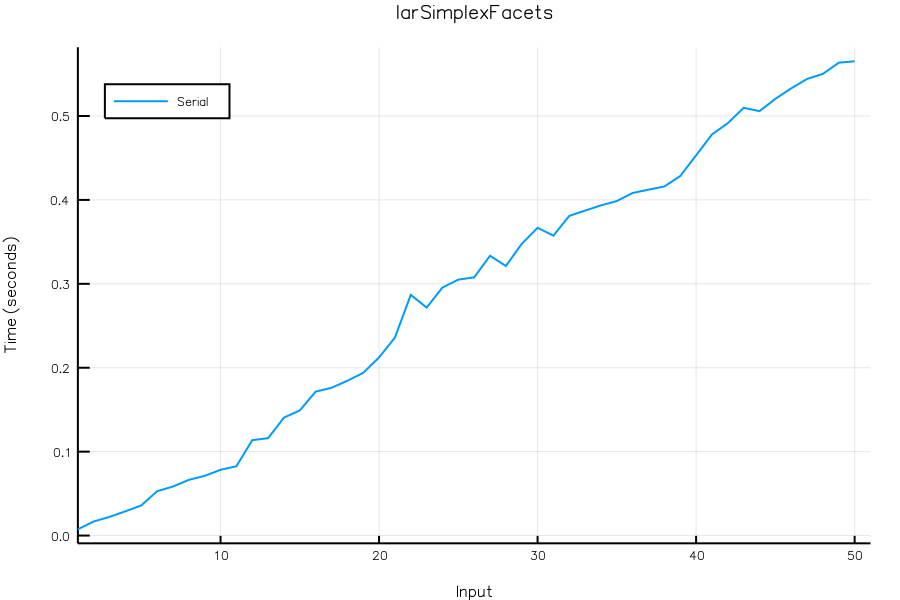
\includegraphics[scale=0.245]{figures/larSimplexFacetsserial}} \quad
\subfloat[][\emph{Parallel}]
	{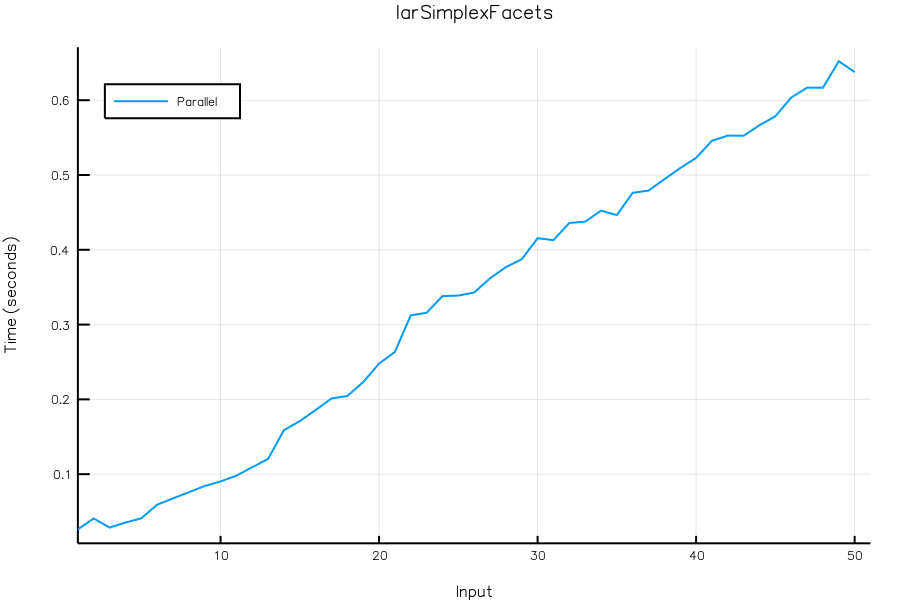
\includegraphics[scale=0.245]{figures/larSimplexFacetsparallel}} \\
\subfloat[][\emph{Both}]
	{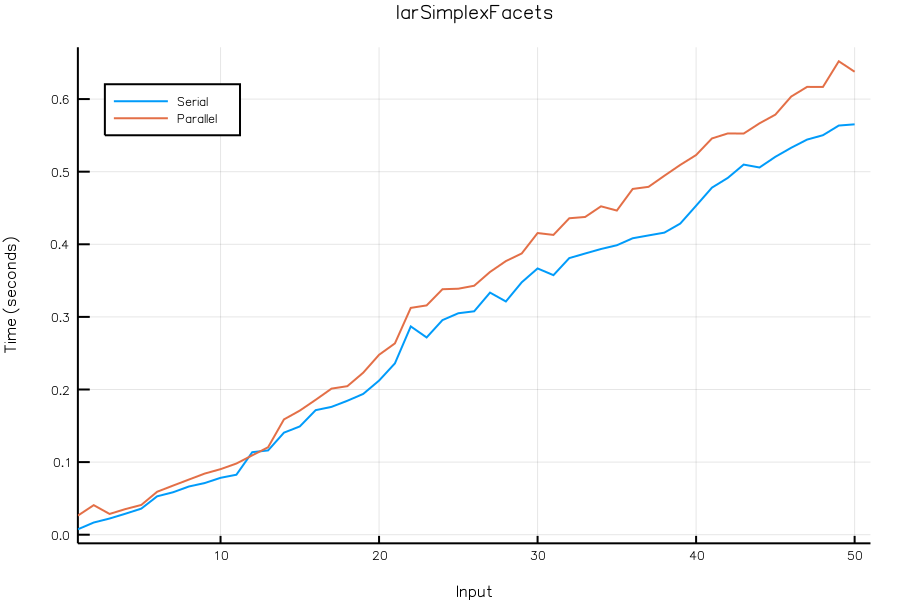
\includegraphics[scale=0.245]{figures/larSimplexFacetsboth}}
\caption{larSimplexFacets}
\label{fig:larSimplexFacets}
\end{figure}


\subsection{quads2tria}
This function gives the conversion of a LAR boundary representation (B-Rep), i.e. a LAR model \textbf{\textsc{V, FV}} made of 2D faces, usually quads but also general polygons, into a LAR model \textbf{\textsc{verts, triangles}} made by triangles.

\subsubsection{Python code}
\begin{verbatim}
def quads2tria(model):
   V,FV = model
   out = []
   nverts = len(V)-1
   for face in FV:
      centroid = CCOMB([V[v] for v in face])
      V += [centroid]
      nverts += 1
      
      v1, v2 = DIFF([V[face[0]],centroid]), DIFF([V[face[1]],centroid])
      v3 = VECTPROD([v1,v2])
      if ABS(VECTNORM(v3)) < 10**3:
         v1, v2 = DIFF([V[face[0]],centroid]), DIFF([V[face[2]],centroid])
         v3 = VECTPROD([v1,v2])
      transf = mat(INV([v1,v2,v3]))
      verts = [(V[v]*transf).tolist()[0][:-1]  for v in face]

      tcentroid = CCOMB(verts)
      tverts = [DIFF([v,tcentroid]) for v in verts]
      rverts = sorted([[ATAN2(vert),v] for vert,v in zip(tverts,face)])
      ord = [pair[1] for pair in rverts]
      ord = ord + [ord[0]]
      edges = [[n,ord[k+1]] for k,n in enumerate(ord[:-1])]
      triangles = [[nverts] + edge for edge in edges]
      out += triangles
   return V,out
\end{verbatim}

\subsubsection{Julia code - serial}
During the translation the \texttt{if} condition was corrected from \texttt{< 10**3} to \texttt{< 1/(10\^{}3)}.

\begin{Verbatim}
# Transformation to triangles by sorting circularly the vertices of faces
function quads2tria{T<:Real}(model::Tuple{Array{Array{T,1},1},Array{
  Array{Int64,1},1}})
	V, FV = model
	if typeof(V) != Array{Array{Float64,1},1}
		V = convert(Array{Array{Float64,1},1},V)
	end
	out = Array{Int64,1}[]
	nverts = length(V)-1
	for face in FV
		arr = [V[v+1] for v in face]
		centroid = sum(arr)/length(arr)
		append!(V,[centroid])
		nverts += 1
		v1, v2 = V[face[1]+1]-centroid, V[face[2]+1]-centroid
		v3 = cross(v1,v2)
		if norm(v3) < 1/(10^3)
			v1, v2 = V[face[1]+1]-centroid, V[face[3]+1]-centroid
			v3 = cross(v1,v2)
		end
		transf = inv(hcat(v1,v2,v3)')
		verts = [(V[v+1]'*transf)'[1:end-1] for v in face]
		tcentroid = sum(verts)/length(verts)
		tverts = [v-tcentroid for v in verts]
		iterator = collect(zip(tverts,face))
		rverts = [[atan2(reverse(iterator[i][1])...),iterator[i][2]] for i in
		  1:length(iterator)]
		rvertsS = sort(rverts,lt=(x,y)->isless(x[1],y[1]))
		ord = [pair[2] for pair in rvertsS]
		append!(ord,ord[1])
		edges = [[i[2],ord[i[1]+1]] for i in enumerate(ord[1:end-1])]
		triangles = [prepend!(edge,nverts) for edge in edges]
		append!(out,triangles)
	end
	return V, out
end
\end{Verbatim}

\subsubsection{Parallel optimization}
The array comprehension was transformed, where possible, into a \texttt{pmap}; it is not possible to parallelize the \texttt{for} with a \texttt{@parallel} because \texttt{append!(V,[centroid])} needs to be computed before the next iteration of the loop.

\subsubsection{Julia code - parallel}
\begin{Verbatim}
# Transformation to triangles by sorting circularly the vertices of faces
@everywhere function pquads2tria{T<:Real}(model::Tuple{Array{Array{T,1},1},Array{
  Array{Int64,1},1}})
	V, FV = model
	if typeof(V) != Array{Array{Float64,1},1}
		V = convert(Array{Array{Float64,1},1},V)
	end
	out = Array{Int64,1}[]
	nverts = length(V)-1
	for face in FV # no parallel
		arr = [V[v+1] for v in face]
		centroid = sum(arr)/length(arr)
		append!(V,[centroid])
		nverts += 1
		v1, v2 = V[face[1]+1]-centroid, V[face[2]+1]-centroid
		v3 = cross(v1,v2)
		if norm(v3) < 1/(10^3)
			v1, v2 = V[face[1]+1]-centroid, V[face[3]+1]-centroid
			v3 = cross(v1,v2)
		end
		transf = inv(hcat(v1,v2,v3)')
		verts = [(V[v+1]'*transf)'[1:end-1] for v in face]
		tcentroid = sum(verts)/length(verts)
		tverts = pmap(x->x-tcentroid,verts)
		iterator = collect(zip(tverts,face))
		rverts = [[atan2(reverse(iterator[i][1])...),iterator[i][2]] for i in
		  1:length(iterator)]
		rvertsS = sort(rverts,lt=(x,y)->isless(x[1],y[1]))
		ord = [pair[2] for pair in rvertsS]
		append!(ord,ord[1])
		edges = [[i[2],ord[i[1]+1]] for i in enumerate(ord[1:end-1])]
		triangles = pmap(x->prepend!(x,nverts),edges)
		append!(out,triangles)
	end
	return V, out
end
\end{Verbatim}

\subsubsection{Unit tests code}
\emph{- Serial Tests -}

\begin{Verbatim}
@testset "quads2tria" begin
	modIn = ([[0,0,0],[0,1,0],[1,0,0],[1,1,0]],[[0,1,2,3]]) # 2D
	modOut = quads2tria(modIn)
	@test typeof(modIn) == Tuple{Array{Array{Int64,1},1},Array{Array{Int64,1},1}}
	@test typeof(modOut) == Tuple{Array{Array{Float64,1},1},Array{Array{Int64,1},1}}
	edges = 2*sum([length(modIn[2][k]) for k in 1:length(modIn[2])])
	EulerChar = length(modOut[1])-edges+length(modOut[2]) # V - E + F
	@test EulerChar == 1
	
	modIn = ([[0,0,0],[0,1,0],[1,0,0],[1,1,0],[0.5,1.5,0]],[[0,1,2,3,4]]) # 2D
	modOut = quads2tria(modIn)
	@test typeof(modIn) == Tuple{Array{Array{Float64,1},1},Array{Array{Int64,1},1}}
	@test typeof(modOut) == Tuple{Array{Array{Float64,1},1},Array{Array{Int64,1},1}}
	edges = 2*sum([length(modIn[2][k]) for k in 1:length(modIn[2])])
	EulerChar = length(modOut[1])-edges+length(modOut[2]) # V - E + F
	@test EulerChar == 1
	
	modIn = ([[0,0,0],[0,1,0],[1,0,0],[1,1,0],[0,0,1],[0,1,1],[1,0,1],[1,1,1]],
	  [[0,1,2,3,4,5,6,7]]) # 3D
	modOut = quads2tria(modIn)
	@test typeof(modIn) == Tuple{Array{Array{Int64,1},1},Array{Array{Int64,1},1}}
	@test typeof(modOut) == Tuple{Array{Array{Float64,1},1},Array{Array{Int64,1},1}}
	edges = 2*sum([length(modIn[2][k]) for k in 1:length(modIn[2])])
	EulerChar = length(modOut[1])-edges+length(modOut[2]) # V - E + F
	@test EulerChar == 1
	
	modIn = ([[0,0,0],[0,1,0],[1,0,0],[1,1,0],[0,0,1],[0,1,1],[1,0,1],[1,1,1],[0.5,0.5,1.5]],
	  [[0,1,2,3,4,5,6,7,8]]) # 3D
	modOut = quads2tria(modIn)
	@test typeof(modIn) == Tuple{Array{Array{Float64,1},1},Array{Array{Int64,1},1}}
	@test typeof(modOut) == Tuple{Array{Array{Float64,1},1},Array{Array{Int64,1},1}}
	edges = 2*sum([length(modIn[2][k]) for k in 1:length(modIn[2])])
	EulerChar = length(modOut[1])-edges+length(modOut[2]) # V - E + F
	@test EulerChar == 1
end
\end{Verbatim}

\emph{- Parallel Tests -}

\begin{Verbatim}
@testset "pquads2tria" begin
	modIn = ([[0,0,0],[0,1,0],[1,0,0],[1,1,0]],[[0,1,2,3]]) # 2D
	modOut = pquads2tria(modIn)
	@test typeof(modIn) == Tuple{Array{Array{Int64,1},1},Array{Array{Int64,1},1}}
	@test typeof(modOut) == Tuple{Array{Array{Float64,1},1},Array{Array{Int64,1},1}}
	edges = 2*sum([length(modIn[2][k]) for k in 1:length(modIn[2])])
	EulerChar = length(modOut[1])-edges+length(modOut[2]) # V - E + F
	@test EulerChar == 1
	
	modIn = ([[0,0,0],[0,1,0],[1,0,0],[1,1,0],[0.5,1.5,0]],[[0,1,2,3,4]]) # 2D
	modOut = pquads2tria(modIn)
	@test typeof(modIn) == Tuple{Array{Array{Float64,1},1},Array{Array{Int64,1},1}}
	@test typeof(modOut) == Tuple{Array{Array{Float64,1},1},Array{Array{Int64,1},1}}
	edges = 2*sum([length(modIn[2][k]) for k in 1:length(modIn[2])])
	EulerChar = length(modOut[1])-edges+length(modOut[2]) # V - E + F
	@test EulerChar == 1
	
	modIn = ([[0,0,0],[0,1,0],[1,0,0],[1,1,0],[0,0,1],[0,1,1],[1,0,1],[1,1,1]],
	  [[0,1,2,3,4,5,6,7]]) # 3D
	modOut = pquads2tria(modIn)
	@test typeof(modIn) == Tuple{Array{Array{Int64,1},1},Array{Array{Int64,1},1}}
	@test typeof(modOut) == Tuple{Array{Array{Float64,1},1},Array{Array{Int64,1},1}}
	edges = 2*sum([length(modIn[2][k]) for k in 1:length(modIn[2])])
	EulerChar = length(modOut[1])-edges+length(modOut[2]) # V - E + F
	@test EulerChar == 1
	
	modIn = ([[0,0,0],[0,1,0],[1,0,0],[1,1,0],[0,0,1],[0,1,1],[1,0,1],[1,1,1],[0.5,0.5,1.5]],
	  [[0,1,2,3,4,5,6,7,8]]) # 3D
	modOut = pquads2tria(modIn)
	@test typeof(modIn) == Tuple{Array{Array{Float64,1},1},Array{Array{Int64,1},1}}
	@test typeof(modOut) == Tuple{Array{Array{Float64,1},1},Array{Array{Int64,1},1}}
	edges = 2*sum([length(modIn[2][k]) for k in 1:length(modIn[2])])
	EulerChar = length(modOut[1])-edges+length(modOut[2]) # V - E + F
	@test EulerChar == 1
end
\end{Verbatim}

\subsubsection{Speedup script code}
\begin{Verbatim}
verts = [[0,0,0],[0,1,0],[1,0,0],[1,1,0],[2,2,0],[2,3,0],[3,2,0],[3,3,0]]
quads = [[0,1,2,3],[4,5,6,7]]
len = length(quads[1])
for k in 2:2*N^2
	append!(verts,verts[end-len+1:end]+1)
	append!(quads,[quads[end]+len])
end
timeSer = [timing(quads2tria,[(verts[1:len*k],quads[1:k])],nt) for k in 1:2*N^2]
timePar = [timing(pquads2tria,[(verts[1:len*k],quads[1:k])],nt) for k in 1:2*N^2]
plotting("quads2tria",timeSer,timePar)
\end{Verbatim}

See figure~\ref{fig:quads2tria}.

\begin{figure}[h]
\centering
\subfloat[][\emph{Serial}]
	{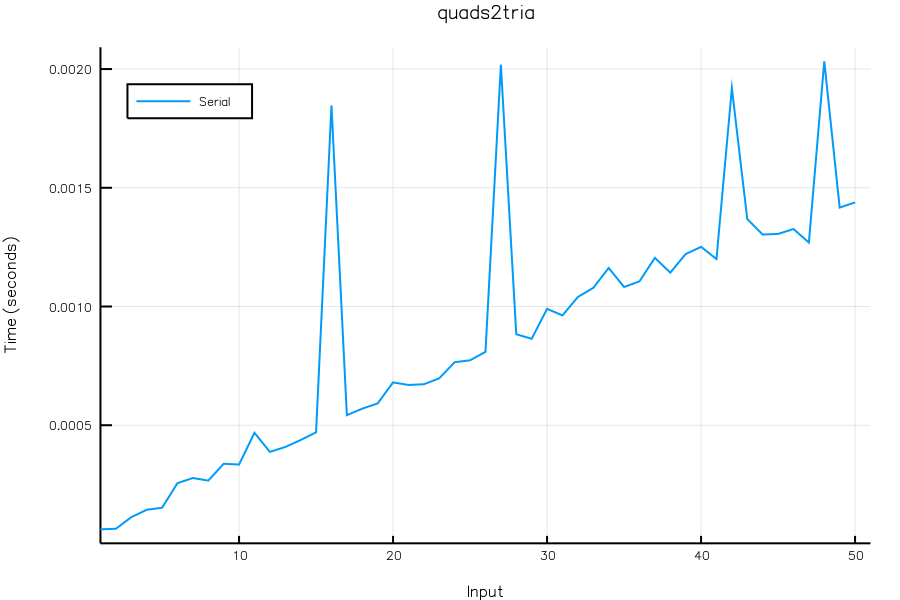
\includegraphics[scale=0.245]{figures/quads2triaserial}} \quad
\subfloat[][\emph{Parallel}]
	{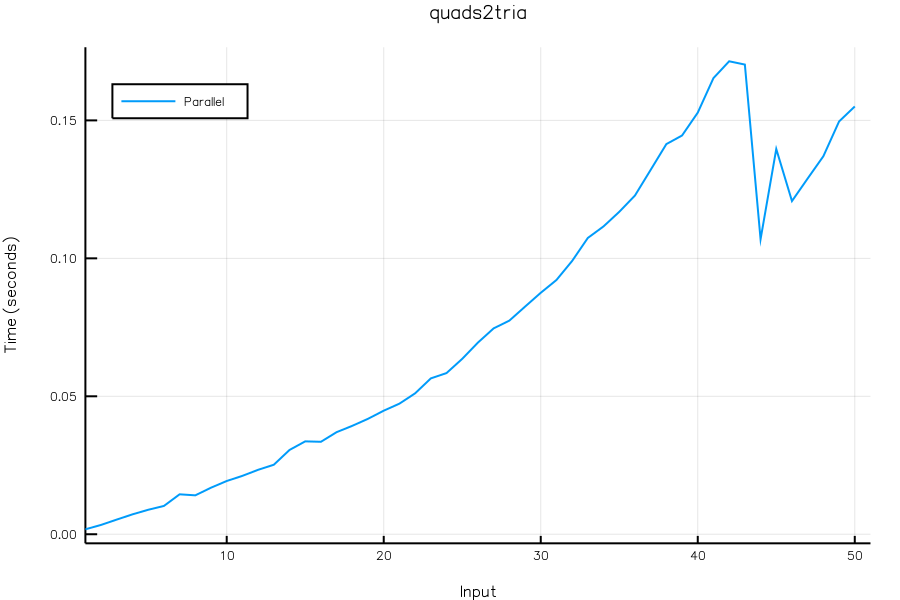
\includegraphics[scale=0.245]{figures/quads2triaparallel}} \\
\subfloat[][\emph{Both}]
	{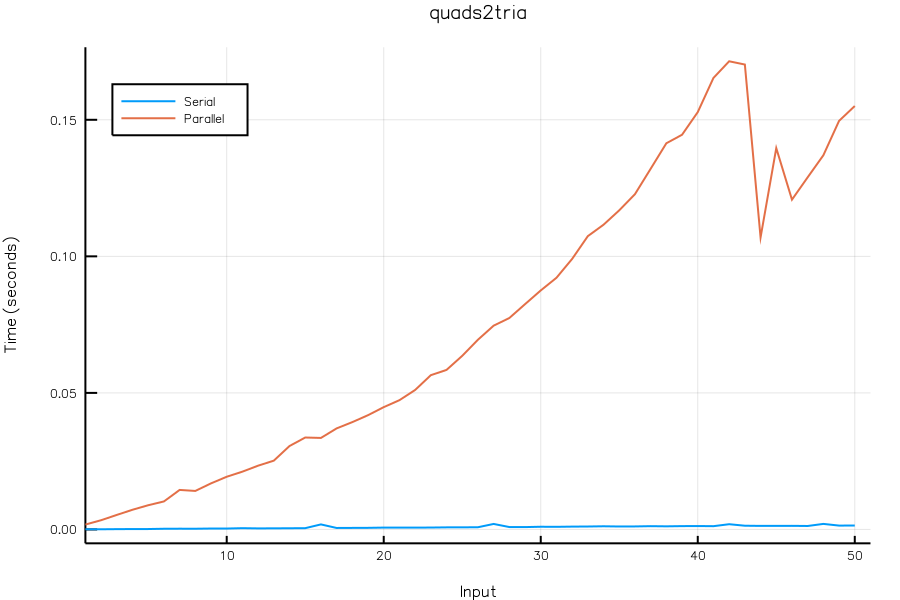
\includegraphics[scale=0.245]{figures/quads2triaboth}}
\caption{quads2tria}
\label{fig:quads2tria}
\end{figure}


% ------- CONCLUSIONS -------
\section{Conclusions}
The \texttt{larExtrude1} function was rethought almost from scratch (to avoid the list nesting of Python and to allow the parallelization process) and in fact it is a lot faster with the increasing of the input size.

The other two parallelized functions have showed the parallel code is not faster than the serial one.
A possible way to address this problem could be to rewrite all the functions using different structures and procedures to handle the data, avoiding array of arrays and similar.
However, the complete lack of documentation online, official and non, for the correct use of the macros and how they specifically work makes the task quite difficult.


% ------- EXAMPLES -------
\clearpage
\thispagestyle{plain}
\appendix
\section{Examples}
The translation of the Python examples and tests is not shown in this report because the code is directly compared with the Python output, which is pretty verbose.

However, the links for the code in the GitHub repository are provided \href{https://github.com/EmaLoprevite/Simplexn/blob/master/test/examples-serial.jl}{here}
and \href{https://github.com/EmaLoprevite/Simplexn/blob/master/test/examples-parallel.jl}{here}, respectively for the serial and the parallel version.


% ------- LIST OF FIGURES -------
\clearpage
\thispagestyle{plain}
\listoffigures

% ------- BIBLIOGRAPHY -------
\clearpage												% clear page for bibliography, if report use cleardoublepage
\thispagestyle{plain}										% not the default page style, empty/plain
\phantomsection										% needed using hyperref
\addcontentsline{toc}{section}{\refname}						% section and refname if article, chapter and bibname if report

\begin{thebibliography}{9}

\bibitem{Paoluzzi:coursewebpage}
IN480 course \href{https://www.dia.uniroma3.it/~paoluzzi/web/did/calcoloparallelo/2018/}{web page}.

\bibitem{Paoluzzi:simplexn}
Python $Simple_{X}^{n}$ module \href{https://github.com/cvdlab/lar-cc/blob/master/doc/pdf/simplexn.pdf}{pdf}.

\bibitem{Paoluzzi:book}
A.~Paoluzzi, \emph{Geometric Programming for Computer-Aided Design}, Wiley, 2003.

\bibitem{Julia:site}
Official \href{https://docs.julialang.org/en/stable/}{Julia Documentation}.

\bibitem{Julia:plots}
Documentation of the \href{https://docs.juliaplots.org/latest/}{Plots package} for Julia.

\bibitem{Sherrington:book}
M.~Sherrington, \emph{Mastering Julia}, Packt Publishing, 2015.

\end{thebibliography}


\end{document}
